% id: 0612
% book: RPM 중3-2 수학 · 06 상관관계
% section: 유형 01 산점도와 상관관계의 뜻
% figure: crop:fig-0612.png
% answer: ①, ④
% answer_source: 답지
% variant_level: 0 (원본 전사)
% 이 파일은 build.mjs 가 items.json 에서 만든다. 고칠 때는 items.json 을 고친다.
\smash{\raisebox{1.5mm}{\dmkichul{대표문제}}}
다음 중 두 변량 $x$, $y$ 사이에 상관관계가 있는 산점도를 모두 고르면? \mbox{(정답 2개)}
\par\smallskip\begin{center}\setlength{\dmfigw}{190.4pt}\ifdim\dmfigw>\linewidth\setlength{\dmfigw}{\linewidth}\fi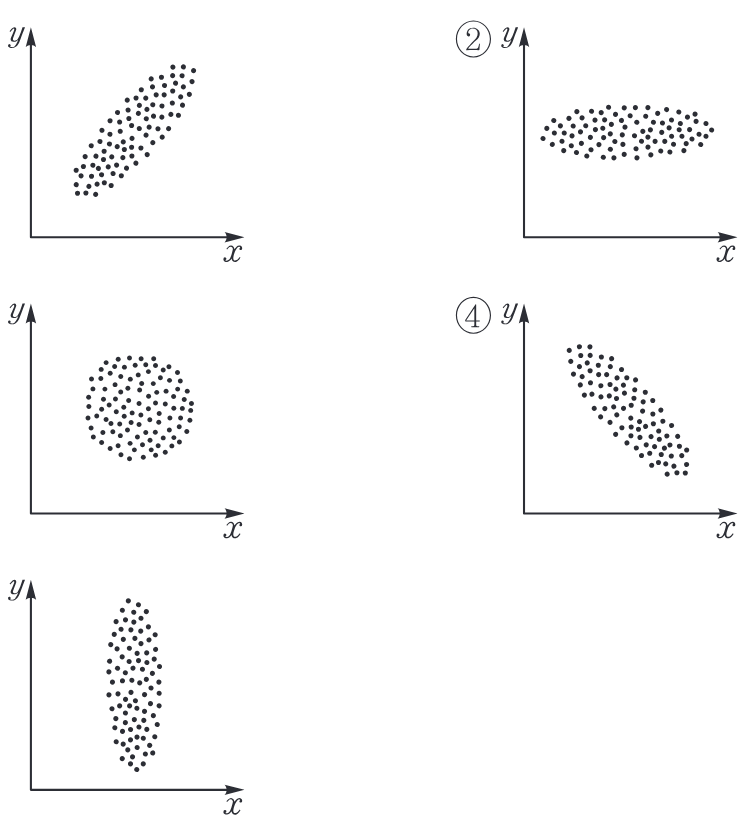
\includegraphics[width=\dmfigw]{figures/fig-0612.png}\end{center}
